% ថ្នាក់ទី ១១ (វិទ្យាសាស្ត្រសង្គម) · ជំពូកទី ៥ · មេរៀនទី ១ · សៀវភៅ ទំព័រ ១៥៣–១៧៣
\chapter{លីមីតនិងដេរីវេ}

\begin{note}[ជំពូកទី ៥ ៖ លីមីតនិងដេរីវេ]
នៅក្នុងជំពូកនេះ គេចាប់ផ្ដើមសិក្សាពីបញ្ញត្តិមូលដ្ឋាននៃលីមីត និងប្រមាណវិធីលើលីមីត ដែលជាមធ្យោបាយដ៏សំខាន់សម្រាប់ឈានទៅសិក្សាបញ្ញត្តិនៃដេរីវេ និងប្រមាណវិធីលើដេរីវេនៃអនុគមន៍ ។ បន្ទាប់ពីទទួលបានបញ្ញត្តិ លីមីត ដេរីវេ និងបំណិនក្នុងការគណនាលីមីត ដេរីវេ គេនឹងអាចប្រើចំណេះដឹង និងបំណិនទាំងនោះក្នុងការដោះស្រាយចំណោទបន្ទាត់ប៉ះនឹងក្រាបតាងអនុគមន៍ត្រង់ចំណុចមួយ ការសិក្សាអថេរភាពសង់ក្រាបតាងអនុគមន៍សនិទានងាយៗ មួយចំនួន ការគណនាតម្លៃអតិបរមាធៀប តម្លៃអប្បបរមាធៀប ការគណនាល្បឿននៃចលនា ហើយលើសពីនេះទៅទៀត គេឈានទៅប្រើក្រាបតាងអនុគមន៍សម្រាប់ដោះស្រាយសមីការ និងវិសមីការមួយចំនួនទៀត ។ ការអនុវត្តទាំងអស់នេះ អាចឆ្លុះបញ្ចាំងឱ្យឃើញពីអត្ថន័យពេញលេញ និងសារប្រយោជន៍នៃគណិតវិទ្យាចំពោះវិទ្យាសាស្ត្រ និងការដោះស្រាយចំណោទបញ្ហាខ្លះក្នុងជីវភាពប្រចាំថ្ងៃ ។
\end{note}

\begin{objBox}[វត្ថុបំណង]
\begin{enumerate}[1]
  \item កំណត់បញ្ញត្តិលីមីតតាមបែបពីជគណិតនិងតាមបែបក្រាប
  \item រកលីមីតនៃផលបូក ផលដក ផលគុណ និងផលចែក
  \item រកលីមីតនៃអនុគមន៍ពហុធានិងអនុគមន៍សនិទាន
  \item រកអត្រាបម្រែបម្រួលមធ្យមនៃអនុគមន៍
  \item កំណត់បញ្ញត្តិដេរីវេនិងធ្វើប្រមាណវិធីលើដេរីវេ ។
\end{enumerate}
\end{objBox}

ក្នុងជំពូកនេះ យើងចាប់ផ្ដើមសិក្សាគណិតវិភាគ សម្រាប់ប្រើក្នុងការដោះស្រាយចំណោទបន្ទាត់ប៉ះ និងចំណោទតម្លៃបរមា ។

\section{លីមីត}
\subsection{សញ្ញាណលីមីត}

\begin{example}[ឧទាហរណ៍ ១]
គេឱ្យអនុគមន៍ $y = f(x) = x^2 + 2x - 3$ និងតារាងតម្លៃលេខ
\[
\begin{array}{c|ccccccc}
x & 1.99 & 1.999 & 1.9999 & \to 2 \leftarrow & 2.0001 & 2.001 & 2.01\\ \hline
y & 4.9401 & 4.9940 & 4.9994 & \to 5 \leftarrow & 5.0006 & 5.0060 & 5.0601
\end{array}
\]
\end{example}
តាមតារាងតម្លៃលេខ បើ $x$ ខិតជិត $2$ ពីខាងឆ្វេង $(x \to 2^-)$ និងពីខាងស្ដាំ $(x \to 2^+)$ នោះ $y$ ខិតជិត $5$ ។ គេថាអនុគមន៍ $y = f(x)$ មានលីមីតស្មើនឹង $5$ កាលណា $x$ ខិតជិត $2$ ។ គេកំណត់សរសេរ
\[
\begin{gathered}
\lim_{x \to 2} f(x) = 5 \quad \text{ឬ}\\
\lim_{x \to 2}(x^2 + 2x - 3) = 5 \text{ ។}
\end{gathered}
\]

\begin{example}[ឧទាហរណ៍ ២]
គេឱ្យអនុគមន៍ $f(x) = \dfrac{x^2 - 9}{x - 3}$ ។ ចំពោះ $x \ne 3$ គេបាន $f(x) = x + 3$ និងក្រាប $L$ ។ តាមក្រាបបើ $x$ ខិតជិត $3$ នោះអនុគមន៍ $y = f(x)$ ខិតជិត $6$ ។ គេកំណត់សរសេរ $\displaystyle\lim_{x \to 3} f(x) = \lim_{x \to 3}\frac{x^2 - 9}{x - 3} = 6$ ។
\end{example}

\begin{center}
\begin{tikzpicture}[scale=0.55]
  \draw[->] (-4,0) -- (5,0) node[right] {$x$};
  \draw[->] (0,-1) -- (0,7.5) node[above] {$y$};
  \draw[thick,red] (-3.5,-0.5) -- (3.8,6.8) node[right] {$L$};
  \draw[dashed] (3,0) -- (3,6) -- (0,6);
  \draw[fill=white] (3,6) circle (3pt);
  \node[below] at (3,0) {$3$}; \node[left] at (0,6) {$6$}; \node[left] at (0,3) {$3$};
  \node[below] at (-3,0) {$-3$}; \node[below left] at (0,0) {$0$};
\end{tikzpicture}
\end{center}

\begin{formulaBox}[ជាទូទៅ]
បើ $x$ ខិតជិត $a$ ហើយអនុគមន៍ $y = f(x)$ ខិតជិតតម្លៃ $b$ ណាមួយនោះ គេកំណត់សរសេរ $\displaystyle\lim_{x \to a} f(x) = b$ ។
\end{formulaBox}

\begin{example}[លំហាត់គំរូ]
\begin{enumerate}[a]
  \item បំពេញតារាងតម្លៃលេខនៃ $\dfrac{1}{x}$ ចំពោះ $x = 0.1;\ 0.01;\ 0.001;\ 0.0001$ និង $x = -0.1;\ -0.01;\ -0.001;\ -0.0001$ ។
  \item ទាញរក $\displaystyle\lim_{x \to 0^+}\frac{1}{x}$ និង $\displaystyle\lim_{x \to 0^-}\frac{1}{x}$ ។
\end{enumerate}
\end{example}
\ans
\begin{enumerate}[a]
  \item តារាងតម្លៃលេខទី $1$ និងទី $2$ ៖
  \[
  \begin{array}{c|ccccc}
  x & 0.1 & 0.01 & 0.001 & 0.0001 & \cdots\\ \hline
  \frac{1}{x} & 10 & 100 & 1000 & 10000 & \cdots
  \end{array}
  \]
  \[
  \begin{array}{c|ccccc}
  x & -0.1 & -0.01 & -0.001 & -0.0001 & \cdots\\ \hline
  \frac{1}{x} & -10 & -100 & -1000 & -10000 & \cdots
  \end{array}
  \]
  \item តាមតារាងតម្លៃលេខទី $1$ គេសង្កេតឃើញថាកាលណា $x$ យកតម្លៃវិជ្ជមាន ហើយកាន់តែតូចទៅៗស្ទើរតែខិតជិតសូន្យ នោះ $\dfrac{1}{x}$ មានតម្លៃវិជ្ជមាន ហើយកាន់តែធំទៅៗគ្មានទីបញ្ចប់ ។ ដូច្នេះ $\displaystyle\lim_{x \to 0^+}\frac{1}{x} = +\infty$ ។

  តាមតារាងតម្លៃលេខទី $2$ គេសង្កេតឃើញថាកាលណា $x$ យកតម្លៃអវិជ្ជមាន ហើយកាន់តែធំទៅៗស្ទើរតែខិតជិតសូន្យ នោះ $\dfrac{1}{x}$ មានតម្លៃអវិជ្ជមានកាន់តែតូចទៅៗគ្មានទីបញ្ចប់ ។ ដូច្នេះ $\displaystyle\lim_{x \to 0^-}\frac{1}{x} = -\infty$ ។
\end{enumerate}

\begin{note}[សម្គាល់]
បើ $x \to a^+$ មានន័យថា $x \to a$ និង $x > a$ ដូចគ្នាដែរ $x \to a^-$ មានន័យថា $x \to a$ និង $x < a$ ។
\end{note}

\begin{pro}
\begin{enumerate}[1]
  \item ក. បំពេញតារាងតម្លៃលេខនៃ $f(x) = \dfrac{x^2 - 4}{x - 2}$ ចំពោះ $x = 1.9;\ 1.99;\ 1.999;\ 2.001;\ 2.01;\ 2.1$ ហើយទាញរក $\displaystyle\lim_{x \to 2} f(x)$ ។ \\ ខ. ចំពោះ $x \ne 2$ ចូរសម្រួលកន្សោម $f(x)$ រួចទាញរកតម្លៃ $\displaystyle\lim_{x \to 2} f(x)$ ។
  \item សង់ក្រាបតាង $g(x) = x^2 + 2$ ហើយទាញរក $\displaystyle\lim_{x \to 1} g(x)$ ។
\end{enumerate}
\ans
\begin{enumerate}[1]
  \item ក. $f(x) = 3.9;\ 3.99;\ 3.999;\ 4.001;\ 4.01;\ 4.1$ នាំឱ្យ $\displaystyle\lim_{x \to 2} f(x) = 4$ \quad ខ. $f(x) = x + 2$ ដូច្នេះ $\displaystyle\lim_{x \to 2} f(x) = 4$
  \item $\displaystyle\lim_{x \to 1} g(x) = 3$ ។
\end{enumerate}
\end{pro}

\subsection{ប្រមាណវិធីលើលីមីត}

អនុគមន៍ $y = f(x)$ និង $y = g(x)$ មានលីមីតកាលណា $x \to a$ ។ គេបាន
\begin{itemize}
  \item $\displaystyle\lim_{x \to a} f(x) = \lim_{x \to a} c = c$ ដែល $f(x) = c$ ជាអនុគមន៍ថេរ
  \item $\displaystyle\lim_{x \to a} f(x) = \lim_{x \to a} x = a$ ដែល $f(x) = x$
  \item $\displaystyle\lim_{x \to a}[f(x) + g(x)] = \lim_{x \to a} f(x) + \lim_{x \to a} g(x)$
  \item $\displaystyle\lim_{x \to a}[f(x) - g(x)] = \lim_{x \to a} f(x) - \lim_{x \to a} g(x)$
  \item $\displaystyle\lim_{x \to a}[f(x)\times g(x)] = \lim_{x \to a} f(x)\times\lim_{x \to a} g(x)$
  \item $\displaystyle\lim_{x \to a}\frac{f(x)}{g(x)} = \frac{\lim_{x \to a} f(x)}{\lim_{x \to a} g(x)}$ បើ $\displaystyle\lim_{x \to a} g(x) \ne 0$ ។
\end{itemize}

\begin{example}[លំហាត់គំរូ ១]
គណនាលីមីតខាងក្រោម ៖ \quad ក. $\displaystyle\lim_{x \to 1}(3 + x)$ \quad ខ. $\displaystyle\lim_{x \to 2}(3x^4)$ ។
\end{example}
\ans
\begin{enumerate}[a]
  \item $\displaystyle\lim_{x \to 1}(3 + x) = \lim_{x \to 1} 3 + \lim_{x \to 1} x = 3 + 1 = 4$ ។
  \item $\displaystyle\lim_{x \to 2}(3x^4) = \lim_{x \to 2} 3\cdot\lim_{x \to 2} x^4 = 3\cdot\lim_{x \to 2} x\cdot\lim_{x \to 2} x\cdot\lim_{x \to 2} x\cdot\lim_{x \to 2} x = 3\cdot 2^4 = 48$ ។
\end{enumerate}

\begin{formulaBox}[ជាទូទៅ]
$\displaystyle\lim_{x \to x_0}(ax^n) = ax_0^n$ ។
\end{formulaBox}

\begin{example}[លំហាត់គំរូ ២]
គណនាលីមីតខាងក្រោម ៖ \quad ក. $\displaystyle\lim_{x \to 1}(x^3 - 3x^2 + x + 1)$ \quad ខ. $\displaystyle\lim_{x \to 3}\frac{x^2 - x + 1}{x - 2}$ ។
\end{example}
\ans
\begin{enumerate}[a]
  \item $\displaystyle\lim_{x \to 1}(x^3 - 3x^2 + x + 1) = \lim_{x \to 1} x^3 - \lim_{x \to 1} 3x^2 + \lim_{x \to 1} x + \lim_{x \to 1} 1 = 1^3 - 3\cdot 1^2 + 1 + 1 = 0$ ។
  \item $\displaystyle\lim_{x \to 3}\frac{x^2 - x + 1}{x - 2} = \frac{\lim_{x \to 3}(x^2 - x + 1)}{\lim_{x \to 3}(x - 2)} = \frac{3^2 - 3 + 1}{3 - 2} = \frac{7}{1} = 7$ ។
\end{enumerate}

\begin{formulaBox}[ជាទូទៅ]
\begin{itemize}
  \item បើ $P(x)$ ជាអនុគមន៍ពហុធានៃ $x$ នោះ $\displaystyle\lim_{x \to x_0} P(x) = P(x_0)$
  \item បើ $\dfrac{f(x)}{g(x)}$ ដែល $g(x) \ne 0$ ជាអនុគមន៍សនិទាន នោះ $\displaystyle\lim_{x \to x_0}\frac{f(x)}{g(x)} = \frac{f(x_0)}{g(x_0)}$ ដែល $g(x_0) \ne 0$ ។
\end{itemize}
\end{formulaBox}

\begin{note}[សម្គាល់]
បើភាគយកនិងភាគបែងមានលីមីតសូន្យនោះ គេត្រូវគណនាតាមជំហានដូចខាងក្រោម ៖
\begin{itemize}
  \item ជំហានទី $1$ ៖ បំបែកភាគយកនិងភាគបែងនៃប្រភាគជាផលគុណកត្តា ។
  \item ជំហានទី $2$ ៖ សម្រួលកត្តារួមចោល ។
  \item ជំហានទី $3$ ៖ រកលីមីតនៃប្រភាគថ្មី ។
\end{itemize}
ក្នុងករណីនេះ គេថាលីមីតមានរាងមិនកំណត់ $\dfrac{0}{0}$ ។
\end{note}

\begin{example}[លំហាត់គំរូ ៣]
គណនាលីមីតខាងក្រោម ៖ \quad ក. $\displaystyle\lim_{x \to -2}\frac{x^2 + 5x + 6}{x^2 - 4}$ \quad ខ. $\displaystyle\lim_{x \to 2}\left(\frac{3x}{x - 2} + \frac{6}{2 - x}\right)$ ។
\end{example}
\ans
\begin{enumerate}[a]
  \item $\displaystyle\lim_{x \to -2}\frac{x^2 + 5x + 6}{x^2 - 4}$ មានរាងមិនកំណត់ $\dfrac{0}{0}$ ។

  ជំហានទី $1$ ៖ $\dfrac{x^2 + 5x + 6}{x^2 - 4} = \dfrac{(x + 2)(x + 3)}{(x + 2)(x - 2)}$ ។ \quad ជំហានទី $2$ ៖ $\dfrac{x^2 + 5x + 6}{x^2 - 4} = \dfrac{x + 3}{x - 2}$ ដែល $x + 2 \ne 0$ ។

  ជំហានទី $3$ ៖ $\displaystyle\lim_{x \to -2}\frac{x^2 + 5x + 6}{x^2 - 4} = \lim_{x \to -2}\frac{x + 3}{x - 2} = \frac{-2 + 3}{-2 - 2} = -\frac{1}{4}$ ។
  \item $\displaystyle\lim_{x \to 2}\left(\frac{3x}{x - 2} + \frac{6}{2 - x}\right) = \lim_{x \to 2}\left(\frac{3x}{x - 2} - \frac{6}{x - 2}\right)$ ដែលមាន $\displaystyle\lim_{x \to 2}(x - 2) = 0$ ។

  ជំហានទី $1$ ៖ $\dfrac{3x}{x - 2} - \dfrac{6}{x - 2} = \dfrac{3x - 6}{x - 2} = \dfrac{3(x - 2)}{x - 2}$ ។ \quad ជំហានទី $2$ ៖ $\dfrac{3x}{x - 2} - \dfrac{6}{x - 2} = 3$ ដែល $x \ne 2$ ។

  ជំហានទី $3$ ៖ $\displaystyle\lim_{x \to 2}\left(\frac{3x}{x - 2} + \frac{6}{2 - x}\right) = \lim_{x \to 2} 3 = 3$ ។
\end{enumerate}

\begin{pro}
គណនាលីមីតខាងក្រោម ៖
\begin{tasks}(3)
  \task $\displaystyle\lim_{x \to 1}[(x^2 + 4x + 2)(3 - x^2)]$
  \task $\displaystyle\lim_{x \to -2}\frac{3x^2 - x - 4}{(2x + 5)^2}$
  \task $\displaystyle\lim_{x \to 1}\frac{2x^2 - 5x + 3}{x^2 + x - 2}$
  \task $\displaystyle\lim_{x \to 3}\frac{x^2 - 9}{x^2 - x - 6}$
  \task $\displaystyle\lim_{x \to 2}\frac{x^3 - 8}{(x - 2)^2}$
  \task $\displaystyle\lim_{x \to 4}\frac{\sqrt{x} - 2}{x^2 - 16}$
\end{tasks}
\ans
ក. $14$ \quad ខ. $10$ \quad គ. $-\dfrac{1}{3}$ \quad ឃ. $\dfrac{6}{5}$ \quad ង. $+\infty$ (ព្រោះ $\dfrac{x^3 - 8}{(x - 2)^2} = \dfrac{x^2 + 2x + 4}{x - 2}$ ៖ $+\infty$ ពេល $x \to 2^+$, $-\infty$ ពេល $x \to 2^-$) \quad ច. $\dfrac{1}{32}$ ។
\end{pro}

\subsection{លីមីតខាងឆ្វេងនិងខាងស្ដាំ}

\begin{example}[ឧទាហរណ៍]
គេឱ្យអនុគមន៍ $y = f(x) = \begin{cases} x^2 & \text{បើ } x \le 1\\ x + 2 & \text{បើ } x > 1 \end{cases}$
\end{example}

\begin{center}
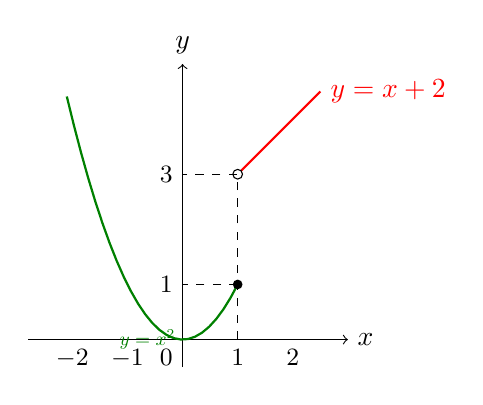
\begin{tikzpicture}[scale=0.7]
  \draw[->] (-2.8,0) -- (3,0) node[right] {$x$};
  \draw[->] (0,-0.5) -- (0,5) node[above] {$y$};
  \draw[thick,green!50!black,domain=-2.1:1] plot (\x,{\x*\x}) node[pos=0.1,left] {$y = x^2$};
  \draw[thick,red] (1,3) -- (2.5,4.5) node[right] {$y = x + 2$};
  \fill (1,1) circle (2.5pt); \draw[fill=white] (1,3) circle (2.5pt);
  \draw[dashed] (1,0) -- (1,3) -- (0,3); \draw[dashed] (1,1) -- (0,1);
  \foreach \x in {-2,-1,1,2} \node[below] at (\x,0) {\small $\x$};
  \foreach \y in {1,3} \node[left] at (0,\y) {\small $\y$};
  \node[below left] at (0,0) {\small $0$};
\end{tikzpicture}
\end{center}

តាមក្រាបគេសង្កេតឃើញថា $f(x)$ ខិតជិត $1$ កាលណា $x$ ខិតជិត $1$ ពីខាងឆ្វេង ។ គេកំណត់សរសេរ $\displaystyle\lim_{x \to 1^-} f(x) = \lim_{x \to 1^-} x^2 = 1$ ។ ម្យ៉ាងទៀត $f(x)$ ខិតជិត $3$ កាលណា $x$ ខិតជិត $1$ ពីខាងស្ដាំ ។ គេកំណត់សរសេរ $\displaystyle\lim_{x \to 1^+} f(x) = \lim_{x \to 1^+}(x + 2) = 3$ ។

\begin{formulaBox}[ជាទូទៅ]
\begin{itemize}
  \item បើ $f(x)$ ខិតជិត $L$ កាលណា $x$ ខិតជិត $x_0$ ពីខាងឆ្វេង នោះ $L$ ជាលីមីតខាងឆ្វេងនៃ $f(x)$ ហើយកំណត់សរសេរ $\displaystyle\lim_{x \to x_0^-} f(x) = L$ ។
  \item បើ $f(x)$ ខិតជិត $R$ កាលណា $x$ ខិតជិត $x_0$ ពីខាងស្ដាំ នោះ $R$ ជាលីមីតខាងស្ដាំនៃ $f(x)$ ហើយកំណត់សរសេរ $\displaystyle\lim_{x \to x_0^+} f(x) = R$ ។
\end{itemize}
\end{formulaBox}

\begin{note}[សម្គាល់]
គេឱ្យអនុគមន៍ $f(x) = \begin{cases} f_1(x) & \text{បើ } x < x_0\\ f_2(x) & \text{បើ } x \ge x_0 \end{cases}$ នោះ $\displaystyle\lim_{x \to x_0^-} f(x) = \lim_{x \to x_0^-} f_1(x)$, \ $\displaystyle\lim_{x \to x_0^+} f(x) = \lim_{x \to x_0^+} f_2(x)$ ។
\end{note}

\begin{example}[លំហាត់គំរូ ១]
គេឱ្យអនុគមន៍ $y = f(x) = \begin{cases} 2x & \text{បើ } x > 0\\ x^3 & \text{បើ } x \le 0 \end{cases}$ ។
\begin{enumerate}[a]
  \item គណនាលីមីត $\displaystyle\lim_{x \to 0^+} f(x)$ និង $\displaystyle\lim_{x \to 0^-} f(x)$ ។
  \item ប្រៀបធៀបតម្លៃលីមីតទាំងពីរ ។
\end{enumerate}
\end{example}
\ans
\begin{enumerate}[a]
  \item $\displaystyle\lim_{x \to 0^+} f(x) = \lim_{x \to 0^+} 2x = 2\times 0 = 0$ និង $\displaystyle\lim_{x \to 0^-} f(x) = \lim_{x \to 0^-} x^3 = 0^3 = 0$ ។
  \item គេមាន $\displaystyle\lim_{x \to 0^+} f(x) = 0$ និង $\displaystyle\lim_{x \to 0^-} f(x) = 0$ ។ ដូច្នេះ $\displaystyle\lim_{x \to 0^+} f(x) = \lim_{x \to 0^-} f(x) = 0$ ។ ក្នុងករណីនេះ គេថាអនុគមន៍ $y = f(x)$ មានលីមីត $0$ ត្រង់ $x = 0$ ។
\end{enumerate}

\begin{example}[លំហាត់គំរូ ២]
គេមានក្រាបតាងអនុគមន៍ $f$ ខាងក្រោម ៖ រក $\displaystyle\lim_{x \to 3^-} f(x)$ និង $\displaystyle\lim_{x \to 3^+} f(x)$ ក្នុងរូបទី $1$, ទី $2$, ទី $3$ និងរូបទី $4$ ។
\end{example}

\begin{center}
\begin{tikzpicture}[scale=0.62]
  \begin{scope}
    \draw[step=1,gray!35] (-1,-3) grid (6,4);
    \draw[->] (-1,0) -- (6,0); \draw[->] (0,-3) -- (0,4);
    \draw[dashed] (3,-3) -- (3,4);
    \draw[thick,blue,domain=-1:2.75,samples=40] plot (\x,{-0.4/(3-\x)+1.5-0.5*\x});
    \draw[thick,blue,domain=3:5.2] plot (\x,{2+0.3*(\x-3)^2});
    \fill[red] (3,2) circle (4pt); \node[below right] at (3,0) {\small $3$};
    \node at (2.5,-4) {\small រូបទី ១};
  \end{scope}
  \begin{scope}[xshift=9cm]
    \draw[step=1,gray!35] (-1,-3) grid (6,4);
    \draw[->] (-1,0) -- (6,0); \draw[->] (0,-3) -- (0,4);
    \draw[dashed] (3,-3) -- (3,4);
    \draw[thick,blue,domain=-1:3] plot (\x,{2-0.25*(\x-3)^2});
    \draw[thick,blue,domain=3:5.3] plot (\x,{-1+0.35*(\x-3)^2+0.2*(\x-3)});
    \fill[red] (3,2) circle (4pt); \fill[red] (3,-1) circle (4pt); \node[below right] at (3,0) {\small $3$};
    \node at (2.5,-4) {\small រូបទី ២};
  \end{scope}
  \begin{scope}[yshift=-9cm]
    \draw[step=1,gray!35] (-1,-3) grid (6,4);
    \draw[->] (-1,0) -- (6,0); \draw[->] (0,-3) -- (0,4);
    \draw[thick,blue,domain=-1:5.5,samples=40] plot (\x,{2-0.06*(\x-3)^3-0.1*(\x-3)});
    \fill[red] (3,2) circle (4pt); \node[below right] at (3,0) {\small $3$};
    \node at (2.5,-4) {\small រូបទី ៣};
  \end{scope}
  \begin{scope}[xshift=9cm,yshift=-9cm]
    \draw[step=1,gray!35] (-1,-3) grid (6,4);
    \draw[->] (-1,0) -- (6,0); \draw[->] (0,-3) -- (0,4);
    \draw[dashed] (3,-3) -- (3,4);
    \draw[thick,blue,domain=-1:3] plot (\x,{3-0.8*(\x-1.2)^2+0.2});
    \draw[thick,blue,domain=3.25:6,samples=40] plot (\x,{0.8/(\x-3)-0.6*(\x-3)});
    \fill[red] (3,{3-0.8*1.8*1.8+0.2}) circle (4pt); \node[below right] at (3,0) {\small $3$};
    \node at (2.5,-4) {\small រូបទី ៤};
  \end{scope}
\end{tikzpicture}
\end{center}
\ans
តាមរូបទី $1$ គេបាន $\displaystyle\lim_{x \to 3^-} f(x) = -\infty$ និង $\displaystyle\lim_{x \to 3^+} f(x) = 2$ ។ \\
តាមរូបទី $2$ គេបាន $\displaystyle\lim_{x \to 3^-} f(x) = 2$ និង $\displaystyle\lim_{x \to 3^+} f(x) = -1$ ។ \\
តាមរូបទី $3$ គេបាន $\displaystyle\lim_{x \to 3^-} f(x) = 2$ និង $\displaystyle\lim_{x \to 3^+} f(x) = 2$ ។ \\
តាមរូបទី $4$ គេបាន $\displaystyle\lim_{x \to 3^-} f(x) = -1$ និង $\displaystyle\lim_{x \to 3^+} f(x) = +\infty$ ។

\begin{formulaBox}[ជាទូទៅ]
អនុគមន៍ $y = f(x)$ មានលីមីតត្រង់ $x_0$ លុះត្រាតែលីមីតខាងឆ្វេងស្មើលីមីតខាងស្ដាំ ។ គេកំណត់សរសេរ $\displaystyle\lim_{x \to x_0^+} f(x) = \lim_{x \to x_0^-} f(x) = \ell$, \ $\ell \in \mathbb{R}$ ។
\end{formulaBox}

\begin{pro}
\begin{enumerate}[a]
  \item គេឱ្យ $f(x) = \begin{cases} 3x + 1 & \text{បើ } x < 2\\ -x + 8 & \text{បើ } x \ge 2 \end{cases}$ ។ គណនា $\displaystyle\lim_{x \to 2^-} f(x)$ និង $\displaystyle\lim_{x \to 2^+} f(x)$ ។
  \item គេឱ្យអនុគមន៍ $y = |x|$ ។ គណនា $\displaystyle\lim_{x \to 0}|x|$ ។ តើអនុគមន៍ $y = |x|$ មានលីមីតត្រង់ $x = 0$ ឬទេ?
  \item គេឱ្យអនុគមន៍ $f(x) = \begin{cases} 5x - 2 & \text{បើ } x < -1\\ -2x + a & \text{បើ } x \ge -1 \end{cases}$ ។ កំណត់តម្លៃ $a$ ដើម្បីឱ្យ $f$ មានលីមីតត្រង់ $x = -1$ ។
\end{enumerate}
\ans
ក. $\displaystyle\lim_{x \to 2^-} f(x) = 7$ និង $\displaystyle\lim_{x \to 2^+} f(x) = 6$ \quad ខ. $\displaystyle\lim_{x \to 0}|x| = 0$ ។ អនុគមន៍ $y = |x|$ មានលីមីតត្រង់ $x = 0$ \quad គ. $a = -9$ ។
\end{pro}

\subsection{លីមីតត្រង់អនន្តនៃអនុគមន៍}
\subsubsection{លីមីតត្រង់អនន្តនៃអនុគមន៍ស្វ័យគុណងាយ}

\begin{example}[ឧទាហរណ៍ ១]
គេឱ្យអនុគមន៍ $y = x^2$ និងតារាងតម្លៃលេខ
\[
\begin{array}{c|cccccc}
x & \cdots & -10^4 & -10^3 & -10^2 & -10 & 0\\ \hline
y = x^2 & \cdots & 10^8 & 10^6 & 10^4 & 10^2 & 0
\end{array}
\]
\[
\begin{array}{c|cccccc}
x & 0 & 10 & 10^2 & 10^3 & 10^4 & \cdots\\ \hline
y = x^2 & 0 & 10^2 & 10^4 & 10^6 & 10^8 & \cdots
\end{array}
\]
\end{example}
តាមតារាងតម្លៃលេខខាងលើ បើ $x$ យកតម្លៃវិជ្ជមានកាន់តែធំទៅៗគ្មានទីបញ្ចប់ នោះអនុគមន៍ $y = x^2$ មានតម្លៃវិជ្ជមានកាន់តែធំទៅៗគ្មានទីបញ្ចប់ដែរ ។ គេថាអនុគមន៍ $y = x^2$ មានលីមីត $+\infty$ កាលណា $x$ ខិតជិត $+\infty$ ហើយគេកំណត់សរសេរ $\displaystyle\lim_{x \to +\infty} x^2 = +\infty$ ។

បើ $x$ យកតម្លៃអវិជ្ជមាន កាន់តែតូចទៅៗគ្មានទីបញ្ចប់ នោះអនុគមន៍ $y = x^2$ មានតម្លៃវិជ្ជមានកាន់តែធំទៅៗគ្មានទីបញ្ចប់ដែរ ។ គេថាអនុគមន៍ $y = x^2$ មានលីមីត $+\infty$ កាលណា $x$ ខិតជិត $-\infty$ ហើយគេកំណត់សរសេរ $\displaystyle\lim_{x \to -\infty} x^2 = +\infty$ ។

\begin{formulaBox}[ជាទូទៅ]
$\displaystyle\lim_{x \to \pm\infty} ax^2 = \begin{cases} +\infty & \text{បើ } a > 0\\ -\infty & \text{បើ } a < 0 \end{cases}$ ។
\end{formulaBox}

\begin{example}[ឧទាហរណ៍ ២]
គេឱ្យអនុគមន៍ $y = \dfrac{1}{x}$ និងតារាងតម្លៃលេខទី $1$ និងទី $2$ ដូចខាងក្រោម ៖
\[
\begin{array}{c|cccccc}
x & 10 & 10^2 & 10^3 & 10^4 & 10^5 & \cdots\\ \hline
y = \frac{1}{x} & 0.1 & 0.01 & 0.001 & 0.0001 & 0.00001 & \cdots
\end{array}
\]
\[
\begin{array}{c|cccccc}
x & -10 & -10^2 & -10^3 & -10^4 & -10^5 & \cdots\\ \hline
y = \frac{1}{x} & -0.1 & -0.01 & -0.001 & -0.0001 & -0.00001 & \cdots
\end{array}
\]
\end{example}
តាមតារាងតម្លៃលេខទី $1$ បើ $x$ យកតម្លៃវិជ្ជមានកាន់តែធំទៅៗគ្មានទីបញ្ចប់ នោះអនុគមន៍ $y = \dfrac{1}{x}$ មានតម្លៃវិជ្ជមានកាន់តែតូចទៅៗជិតស្មើសូន្យ ។ គេថាអនុគមន៍ $y = \dfrac{1}{x}$ មានលីមីតសូន្យ កាលណា $x$ ខិតជិត $+\infty$ ហើយគេកំណត់សរសេរ $\displaystyle\lim_{x \to +\infty}\frac{1}{x} = 0$ ។

តាមតារាងតម្លៃលេខទី $2$ បើ $x$ យកតម្លៃអវិជ្ជមានកាន់តែតូចទៅៗគ្មានទីបញ្ចប់ នោះអនុគមន៍ $y = \dfrac{1}{x}$ មានតម្លៃដាច់ខាតកាន់តែតូចទៅៗជិតស្មើសូន្យ ។ គេកំណត់សរសេរ $\displaystyle\lim_{x \to -\infty}\frac{1}{x} = 0$ ។ ដូច្នេះ $\displaystyle\lim_{x \to \pm\infty}\frac{1}{x} = 0$ ។

\begin{formulaBox}[ជាទូទៅ]
$\displaystyle\lim_{x \to \pm\infty}\frac{a}{x} = 0$ \ $(a \in \mathbb{R})$ ។
\end{formulaBox}

\begin{example}[លំហាត់គំរូ ១]
គណនាលីមីត $\displaystyle\lim_{x \to -\infty} x^3$ និង $\displaystyle\lim_{x \to +\infty}(-2x^3)$ ។
\end{example}
\ans
$\displaystyle\lim_{x \to -\infty} x^3 = \left(\lim_{x \to -\infty} x\right)^3 = -\infty$ និង $\displaystyle\lim_{x \to +\infty}(-2x^3) = -2\left(\lim_{x \to +\infty} x\right)^3 = -\infty$ ។

\begin{example}[លំហាត់គំរូ ២]
គណនាលីមីត $\displaystyle\lim_{x \to \pm\infty}\frac{1}{x^2}$ និង $\displaystyle\lim_{x \to \pm\infty}\frac{4}{x^3}$ ។
\end{example}
\ans
$\displaystyle\lim_{x \to \pm\infty}\frac{1}{x^2} = \frac{1}{\left(\lim_{x \to \pm\infty} x\right)^2} = 0$ និង $\displaystyle\lim_{x \to \pm\infty}\frac{4}{x^3} = \frac{4}{\left(\lim_{x \to \pm\infty} x\right)^3} = 0$ ។

\begin{pro}
គណនាលីមីត \quad ក. $\displaystyle\lim_{x \to \pm\infty}(4x^2)$ \quad ខ. $\displaystyle\lim_{x \to \pm\infty}(-3x^2)$ \quad គ. $\displaystyle\lim_{x \to \pm\infty}\left(-\frac{2}{x^2}\right)$ ។
\ans
ក. $+\infty$ \quad ខ. $-\infty$ \quad គ. $0$ ។
\end{pro}

\subsubsection{លីមីតមានរាងមិនកំណត់ \texorpdfstring{$\infty - \infty$}{inf - inf}}

\begin{example}[ឧទាហរណ៍]
គណនា $\displaystyle\lim_{x \to +\infty}(x^2 - x + 1)$ ។
\end{example}
បើ $x \to +\infty$ នោះ $\displaystyle\lim_{x \to +\infty}(x^2 - x + 1)$ មានរាងមិនកំណត់ $\infty - \infty$ ព្រោះ $\displaystyle\lim_{x \to +\infty} x^2 = +\infty$, $\displaystyle\lim_{x \to +\infty}(-x + 1) = -\infty$ ។

ជំហានទី $1$ ៖ ដាក់តួដែលមានដឺក្រេធំជាងគេជាកត្តារួម $x^2 - x + 1 = x^2\left(1 - \dfrac{1}{x} + \dfrac{1}{x^2}\right)$ ។

ជំហានទី $2$ ៖ រកលីមីតនៃកន្សោមថ្មី
\[
\begin{aligned}
\lim_{x \to +\infty}(x^2 - x + 1) &= \lim_{x \to +\infty}\left[x^2\left(1 - \frac{1}{x} + \frac{1}{x^2}\right)\right]\\
&= \lim_{x \to +\infty} x^2 = +\infty
\end{aligned}
\]
ព្រោះ $\displaystyle\lim_{x \to +\infty}\frac{1}{x} = 0$, $\displaystyle\lim_{x \to +\infty}\frac{1}{x^2} = 0$ ។

\begin{formulaBox}[ជាទូទៅ]
\begin{itemize}
  \item បើលីមីតនៃអនុគមន៍ពហុធាមានរាងមិនកំណត់ $\infty - \infty$ នៅត្រង់អនន្ត នោះគេត្រូវ ៖ ជំហានទី $1$ ៖ ដាក់តួដែលមានដឺក្រេធំជាងគេជាកត្តារួម ។ ជំហានទី $2$ ៖ គណនាលីមីតនៃកន្សោមថ្មី ។
  \item លីមីតនៃអនុគមន៍ពហុធានៅត្រង់អនន្ត គឺជាលីមីតនៃតួដែលមានដឺក្រេធំជាងគេ ។
\end{itemize}
\end{formulaBox}

\begin{pro}
គណនាលីមីតខាងក្រោម ៖ \quad ក. $\displaystyle\lim_{x \to \pm\infty}(x^2 - 2x + 3)$ \quad ខ. $\displaystyle\lim_{x \to -\infty}(2x^3 + x^2 - 3x + 1)$ ។
\ans
ក. $+\infty$ \quad ខ. $-\infty$ ។
\end{pro}

\subsubsection{លីមីតមានរាងមិនកំណត់ \texorpdfstring{$\frac{\infty}{\infty}$}{inf/inf}}

\begin{example}[ឧទាហរណ៍]
គណនា $\displaystyle\lim_{x \to +\infty}\frac{2x + 1}{x - 2}$ និង $\displaystyle\lim_{x \to -\infty}\frac{2x + 1}{x - 2}$ ។
\end{example}
បើ $x$ ខិតជិត $+\infty$ នោះ $\displaystyle\lim_{x \to +\infty}\frac{2x + 1}{x - 2}$ មានរាងមិនកំណត់ $\dfrac{\infty}{\infty}$ ។

ជំហានទី $1$ ៖ ដាក់តួដែលមានដឺក្រេធំជាងគេនៃភាគយក និងភាគបែងជាកត្តារួម ហើយសម្រួលកត្តារួមចោល
\[
\begin{gathered}
\frac{2x + 1}{x - 2} = \frac{x\left(2 + \frac{1}{x}\right)}{x\left(1 - \frac{2}{x}\right)} = \frac{2 + \frac{1}{x}}{1 - \frac{2}{x}},\\
x \ne 0
\end{gathered}
\]
ជំហានទី $2$ ៖ រកលីមីតនៃប្រភាគថ្មី $\displaystyle\lim_{x \to +\infty}\frac{2x + 1}{x - 2} = \lim_{x \to +\infty}\frac{2 + \frac{1}{x}}{1 - \frac{2}{x}} = \frac{2 + 0}{1 - 0} = 2$ ។

តាមរបៀបដូចគ្នា គេបាន $\displaystyle\lim_{x \to -\infty}\frac{2x + 1}{x - 2} = 2$ ។

\begin{formulaBox}[ជាទូទៅ]
\begin{itemize}
  \item បើលីមីតនៃអនុគមន៍សនិទានមានរាងមិនកំណត់ $\dfrac{\infty}{\infty}$ នៅត្រង់អនន្ត នោះគេត្រូវ ៖ ជំហានទី $1$ ៖ ដាក់តួដែលមានដឺក្រេធំជាងគេនៃភាគយក និងភាគបែងជាកត្តារួម ហើយសម្រួលចោល ។ ជំហានទី $2$ ៖ គណនាលីមីតនៃប្រភាគថ្មី ។
  \item លីមីតនៃអនុគមន៍សនិទាននៅត្រង់អនន្ត គឺជាផលធៀបរវាងលីមីតនៃតួដែលមានដឺក្រេធំជាងគេនៅភាគយកនិងលីមីតនៃតួដែលមានដឺក្រេធំជាងគេនៅភាគបែង ។
\end{itemize}
\end{formulaBox}

\begin{pro}
គណនាលីមីត
\begin{tasks}(4)
  \task $\displaystyle\lim_{x \to +\infty}\frac{4 - x}{2x - 1}$
  \task $\displaystyle\lim_{x \to -\infty}\frac{2x - 1}{x^2 + 2}$
  \task $\displaystyle\lim_{x \to -\infty}\frac{x^2 - 2}{x - 1}$
  \task $\displaystyle\lim_{x \to +\infty}\frac{5 - 2x}{x^2 + 3}$
\end{tasks}
\ans
ក. $-\dfrac{1}{2}$ \quad ខ. $0$ \quad គ. $-\infty$ \quad ឃ. $0$ ។
\end{pro}

\section{ដេរីវេ}
\subsection{អត្រាបម្រែបម្រួលមធ្យម}

\begin{example}[ឧទាហរណ៍]
ក្នុងទម្លាក់សេរីនៃវត្ថុមួយ គេបានចម្ងាយចរ $S(t) = 4.9t^2$ ម៉ែត្រ បន្ទាប់ពី $t$ វិនាទីក្រោយមក ។ ល្បឿនមធ្យមនៃទម្លាក់នោះ ក្នុងចន្លោះខណៈ $t_1 = 1\,s$ និង $t_2 = 3\,s$ កំណត់ដោយផលធៀប $\dfrac{\Delta S}{\Delta t}$ ដូចខាងក្រោម ៖
\[
\begin{aligned}
\frac{\Delta S}{\Delta t} &= \frac{S(3) - S(1)}{3 - 1} = \frac{4.9\times 3^2 - 4.9\times 1^2}{2}\\
&= 19.6 \ (m/s)
\end{aligned}
\]
\end{example}
ល្បឿនមធ្យម $\dfrac{\Delta S}{\Delta t}$ ហៅថាអត្រាបម្រែបម្រួលមធ្យមនៃចម្ងាយចរ $S(t)$ ពីខណៈ $t_1$ ទៅខណៈ $t_2$ ។

\begin{formulaBox}[ជាទូទៅ]
បើអថេរ $x$ ប្រែប្រួលពី $a$ ទៅ $b$ ហើយអនុគមន៍ $y = f(x)$ ប្រែប្រួលពី $f(a)$ ទៅ $f(b)$ នោះផលធៀប $\dfrac{\Delta y}{\Delta x} = \dfrac{f(b) - f(a)}{b - a}$ ហៅថាអត្រាបម្រែបម្រួលមធ្យមនៃ $y = f(x)$ កាលណា $x$ ប្រែប្រួលពី $a$ ទៅ $b$ ។
\end{formulaBox}

\begin{example}[លំហាត់គំរូ]
រកអត្រាបម្រែបម្រួលមធ្យមនៃប្រាក់ចំណូល $R(x) = x^2 + 5x$ គិតជាពាន់រៀលនៃការលក់ស្រូវ $x$ តោន កាលណា $x$ ប្រែប្រួលពី $10$ តោនទៅ $13$ តោន ។
\end{example}
\ans
គេបានអត្រាបម្រែបម្រួលមធ្យមនៃប្រាក់ចំណូល
\[ \begin{aligned}
\frac{\Delta R}{\Delta x} &= \frac{R(13) - R(10)}{13 - 10}\\
&= \frac{(13^2 + 5\times 13) - (10^2 + 5\times 10)}{3}\\
&= \frac{84}{3} = 28 \text{ ពាន់រៀលក្នុង } 1 \text{ តោន ។}
\end{aligned} \]

\begin{pro}
\begin{enumerate}[a]
  \item ក្នុងការឃោសនាពាណិជ្ជកម្ម $x$ ថ្ងៃ គេលក់ដាច់ទស្សនាវដ្ដីបានចំនួន $S(x) = x^2 + 20x + 200$ ក្បាល ។ រកអត្រាបម្រែបម្រួលមធ្យមនៃ $S(x)$ ក្នុងរយៈពេលពី $x = 5$ ទៅ $x = 10$ ថ្ងៃ ។
  \item រកអត្រាបម្រែបម្រួលមធ្យមនៃអនុគមន៍ $f(x) = x^3 - 1$ កាលណា $x$ ប្រែប្រួលពី $a$ ទៅ $a + h$ ។
\end{enumerate}
\ans
ក. $35$ \quad ខ. $3a^2 + 3ah + h^2$ ។
\end{pro}

\subsection{ដេរីវេត្រង់ចំណុចមួយ}

\begin{example}[ឧទាហរណ៍]
គេប៉ាន់ស្មានថាក្នុង $x$ ឆ្នាំទៀតប្រជាជននៅក្នុងតំបន់មួយនឹងមានចំនួន $P(x) = x^2 + 20x + 80000$ នាក់ ។
\end{example}
បើ $x$ បម្រែបម្រួលពី $x_1 = 1$ ឆ្នាំ ទៅ $x_2 = a$ ឆ្នាំ នោះគេបានអត្រាបម្រែបម្រួលមធ្យម
\[ \begin{aligned}
\frac{\Delta P}{\Delta x} &= \frac{P(a) - P(1)}{a - 1}\\
&= \frac{(a^2 + 20a + 80000) - (1^2 + 20\times 1 + 80000)}{a - 1}\\
&= \frac{(a - 1)(a + 1) + 20(a - 1)}{a - 1} = a + 21
\end{aligned} \]
បើចន្លោះឆ្នាំ $\Delta x$ កាន់តែតូច $(\Delta x \to 0)$ នោះអត្រាបម្រែបម្រួលមធ្យម $\dfrac{\Delta P}{\Delta x}$ ខិតជិតតម្លៃមួយដែលហៅថាអត្រាបម្រែបម្រួលខណៈ ហើយកំណត់ដោយ
\[
\begin{aligned}
\lim_{\Delta x \to 0}\frac{\Delta P}{\Delta x} &= \lim_{a \to 1}\frac{P(a) - P(1)}{a - 1}\\
&= \lim_{a \to 1}(a + 21) = 22
\end{aligned}
\]
អត្រាបម្រែបម្រួលខណៈ $\displaystyle\lim_{\Delta x \to 0}\frac{\Delta P}{\Delta x} = 22$ ហៅថាដេរីវេនៃអនុគមន៍ $P(x)$ ត្រង់ $x = 1$ ហើយកំណត់សរសេរ $P'(1) = 22$ ។

\begin{formulaBox}[ជាទូទៅ]
ដេរីវេនៃអនុគមន៍ $y = f(x)$ នៅត្រង់ $x = a$ កំណត់ដោយ
\[
\begin{gathered}
f'(a) = \lim_{x \to a}\frac{f(x) - f(a)}{x - a} \quad \text{ឬ}\\
f'(a) = \lim_{h \to 0}\frac{f(a + h) - f(a)}{h}
\end{gathered}
\]
ដែល $x = a + h$ ឬ $h = x - a$ ។
\end{formulaBox}

\begin{example}[លំហាត់គំរូ]
រកដេរីវេនៃអនុគមន៍ $f(x) = x^3$ នៅត្រង់ $x = 1$ ។
\end{example}
\ans
ជំហានទី $1$ ៖ រក $f(1) = 1^3 = 1$ ។

ជំហានទី $2$ ៖ រក $\dfrac{f(1 + h) - f(1)}{h} = \dfrac{(1 + h)^3 - 1^3}{h} = \dfrac{(1 + h - 1)[(1 + h)^2 + (1 + h) + 1]}{h} = (1 + h)^2 + h + 2$ ។

ជំហានទី $3$ ៖ រក $\displaystyle\lim_{h \to 0}\frac{f(1 + h) - f(1)}{h} = \lim_{h \to 0}[(1 + h)^2 + h + 2] = (1 + 0)^2 + 0 + 2 = 3$ ។ ដូច្នេះ $f'(1) = 3$ ។

\begin{pro}
រកដេរីវេនៃអនុគមន៍ខាងក្រោម ៖
\begin{tasks}(3)
  \task $f(x) = -x^2 + 4x$ នៅត្រង់ $x = -1$
  \task $g(x) = x^2 - 4x + 5$ នៅត្រង់ $x = 2$
  \task $y = x^3 - 2$ នៅត្រង់ $x = 0$
\end{tasks}
\ans
ក. $6$ \quad ខ. $0$ \quad គ. $0$ ។
\end{pro}

\subsection{ដេរីវេ}

\begin{example}[ឧទាហរណ៍]
គេឱ្យអនុគមន៍ $f(x) = x^3$ ។
\end{example}
គេបាន $f(a + h) - f(a) = (a + h)^3 - a^3 = (a + h - a)[(a + h)^2 + (a + h)a + a^2] = h[(a + h)^2 + a(a + h) + a^2]$
\[
\begin{aligned}
\lim_{h \to 0}\frac{f(a + h) - f(a)}{h} &\\
&= \lim_{h \to 0}\frac{h[(a + h)^2 + a(a + h) + a^2]}{h}
\end{aligned}
\]
\[ f'(a) = \lim_{h \to 0}[(a + h)^2 + a(a + h) + a^2] = 3a^2 \]
ដោយ $f'(a) = 3a^2$ ចំពោះចំនួនពិត $a$ ណាមួយ នោះគេអាចជំនួស $a$ ដោយចំនួនពិត $x$ ហើយកំណត់សរសេរ $f'(x) = 3x^2$ ។ $f'(x) = 3x^2$ ជាអនុគមន៍ថ្មីមួយទៀត ហើយហៅថាដេរីវេនៃអនុគមន៍ $f(x) = x^3$ ។

\begin{definition}[និយមន័យ]
ដេរីវេនៃអនុគមន៍ $f(x)$ គឺជាអនុគមន៍ដែលកំណត់ដោយ $\displaystyle f'(x) = \lim_{h \to 0}\frac{f(x + h) - f(x)}{h}$ ។ គេអាចប្រើនិមិត្តសញ្ញា $y'$, $\dfrac{dy}{dx}$, $\dfrac{d}{dx}f(x)$ សម្រាប់តាងដេរីវេនៃ $y = f(x)$ ។
\end{definition}

\begin{example}[លំហាត់គំរូ]
គេឱ្យអនុគមន៍ $f(x) = x^2 + 3x$ ។ \quad ក. រកដេរីវេនៃ $f'(x)$ \quad ខ. រក $f'(0)$ និង $f'(-1)$ ។
\end{example}
\ans
\begin{enumerate}[a]
  \item ជំហានទី $1$ ៖ $f(x + h) - f(x) = [(x + h)^2 + 3(x + h)] - (x^2 + 3x) = 2xh + 3h + h^2$ ។

  ជំហានទី $2$ ៖ $\displaystyle\lim_{h \to 0}\frac{f(x + h) - f(x)}{h} = \lim_{h \to 0}\frac{2xh + 3h + h^2}{h} = \lim_{h \to 0}(2x + 3 + h) = 2x + 3$ ។ ដូច្នេះ $f'(x) = 2x + 3$ ។
  \item $f'(0) = 2\times 0 + 3 = 3$, \ $f'(-1) = 2(-1) + 3 = 1$ ។
\end{enumerate}

\begin{pro}
\begin{enumerate}[a]
  \item រកដេរីវេនៃអនុគមន៍ $f(x) = 3x^2$ ហើយទាញរក $f'(1)$ និង $f'(-2)$ ។
  \item រកដេរីវេនៃ $g(x) = 2x^3 - 1$ ហើយទាញរកដេរីវេត្រង់ $x = 0$ និង $x = -1$ ។
\end{enumerate}
\ans
ក. $f'(x) = 6x$, $f'(1) = 6$ និង $f'(-2) = -12$ \quad ខ. $g'(x) = 6x^2$, $g'(0) = 0$ និង $g'(-1) = 6$ ។
\end{pro}

\subsection{រូបមន្តដេរីវេ}
\subsubsection{ដេរីវេនៃអនុគមន៍ថេរ អនុគមន៍ស្វ័យគុណងាយ និងដេរីវេនៃផលគុណចំនួនថេរនឹងអនុគមន៍}

\begin{itemize}
  \item ចំពោះអនុគមន៍ថេរ $f(x) = c$ គេបាន $\displaystyle f'(x) = \lim_{h \to 0}\frac{f(x + h) - f(x)}{h} = \lim_{h \to 0}\frac{c - c}{h} = \lim_{h \to 0} 0 = 0$ ។ ដូច្នេះ បើ $f(x) = c$ នោះ $f'(x) = 0$ ។
  \item ចំពោះអនុគមន៍ស្វ័យគុណងាយ $f(x) = x^n$ ដែល $n \in \mathbb{N}$ គេបាន $f(x + h) - f(x) = (x + h)^n - x^n$ ។ តាង $u = x + h$ ហើយ $h = u - x$ ។ បើ $h \to 0$ នោះ $u \to x$ ។ គេបាន
  \[ \begin{aligned}
f(x + h) - f(x) &= u^n - x^n\\
&= (u - x)(u^{n-1} + u^{n-2}x + \dots + x^{n-1})\\
&= h(u^{n-1} + u^{n-2}x + \dots + x^{n-1})
\end{aligned} \]
  \[ \begin{aligned}
f'(x) &= \lim_{h \to 0}\frac{f(x + h) - f(x)}{h}\\
&= \lim_{u \to x}(u^{n-1} + u^{n-2}x + \dots + x^{n-1})\\
&= \underbrace{x^{n-1} + x^{n-1} + \dots + x^{n-1}}_{n \text{ តួ}} = nx^{n-1}
\end{aligned} \]
  ដូច្នេះ បើ $f(x) = x^n$ នោះ $f'(x) = nx^{n-1}$ ។
  \item ចំពោះអនុគមន៍ផលគុណចំនួនថេរនឹងអនុគមន៍ $y = kf(x)$, $k \in \mathbb{R}$ គេបាន
  \[
\begin{aligned}
y' &= \lim_{h \to 0}\frac{kf(x + h) - kf(x)}{h}\\
&= k\lim_{h \to 0}\frac{f(x + h) - f(x)}{h} = kf'(x)
\end{aligned}
\]
  ដូច្នេះ បើ $y = kf(x)$ នោះ $y' = kf'(x)$ ។
\end{itemize}

\begin{example}[លំហាត់គំរូ]
គណនាដេរីវេនៃអនុគមន៍ \quad ក. $y = 8$ \quad ខ. $y = x^3$ \quad គ. $y = -2x^4$ ។
\end{example}
\ans
ក. $y = 8$ នោះ $y' = (8)' = 0$ \quad ខ. $y = x^3$ នោះ $y' = (x^3)' = 3x^{3-1} = 3x^2$ \quad គ. $y = -2x^4$ នោះ $y' = (-2x^4)' = (-2)(4)x^{4-1} = -8x^3$ ។

\begin{pro}
គណនាដេរីវេនៃអនុគមន៍ \quad ក. $y = -\dfrac{2007}{2008}$ \quad ខ. $y = -x^2$ \quad គ. $y = \dfrac{3}{5}x^5$ ។
\ans
ក. $0$ \quad ខ. $-2x$ \quad គ. $3x^4$ ។
\end{pro}

\subsubsection{ដេរីវេផលបូកនិងផលដកអនុគមន៍}

\begin{itemize}
  \item ចំពោះផលបូកនៃអនុគមន៍ $y = f(x) + g(x)$ ។ គេតាង $F(x) = f(x) + g(x)$ ។ គេបាន
  \[ \begin{aligned}
F(x + h) - F(x) &= [f(x + h) + g(x + h)]\\
&\quad - [f(x) + g(x)]\\
&= [f(x + h) - f(x)] + [g(x + h) - g(x)]
\end{aligned} \]
  \[ \begin{aligned}
y' &= \lim_{h \to 0}\frac{F(x + h) - F(x)}{h}\\
&= \lim_{h \to 0}\frac{f(x + h) - f(x)}{h}\\
&\quad + \lim_{h \to 0}\frac{g(x + h) - g(x)}{h}\\
&= f'(x) + g'(x)
\end{aligned} \]
  ដូច្នេះ បើ $y = f(x) + g(x)$ នោះ $y' = f'(x) + g'(x)$ ។
  \item ចំពោះផលដកនៃអនុគមន៍ $y = f(x) - g(x)$ ។ គេបាន $y = f(x) + (-1)g(x)$ នោះ $y' = f'(x) + [(-1)g(x)]' = f'(x) + (-1)g'(x) = f'(x) - g'(x)$ ។ ដូច្នេះ បើ $y = f(x) - g(x)$ នោះ $y' = f'(x) - g'(x)$ ។
\end{itemize}

\begin{example}[លំហាត់គំរូ]
គណនាដេរីវេនៃអនុគមន៍
\begin{enumerate}[a]
  \item $y = x^2 + 4x$ ហើយទាញរក $y'(0)$ និង $y'(-2)$
  \item $y = x^3 - 3x^2$ ហើយទាញរកដេរីវេត្រង់ $x = 1$ និង $x = -1$
  \item $y = x^4 - 2x^2 + 3x - 2$ ហើយទាញរក $y'(0)$ ។
\end{enumerate}
\end{example}
\ans
\begin{enumerate}[a]
  \item $y' = (x^2)' + (4x)' = 2x + 4$, \ $y'(0) = 2\times 0 + 4 = 4$, \ $y'(-2) = 2(-2) + 4 = 0$ ។
  \item $y' = (x^3)' - (3x^2)' = 3x^2 - 6x$, \ $y'(1) = 3\times 1^2 - 6\times 1 = -3$, \ $y'(-1) = 3(-1)^2 - 6(-1) = 9$ ។
  \item $y' = (x^4)' - (2x^2)' + (3x)' - (2)' = 4x^3 - 4x + 3$, \ $y'(0) = 4\times 0^3 - 4\times 0 + 3 = 3$ ។
\end{enumerate}

\begin{pro}
\begin{enumerate}[a]
  \item គណនា $f'(x)$ និង $f'(1)$ នៃអនុគមន៍ $y = f(x) = \dfrac{x^4}{2} + 2x$ ។
  \item គណនា $y'$, $y'(0)$ និង $y'(1)$ នៃ $y = \dfrac{1}{3}x^3 - x^2$ ។
  \item គណនា $\dfrac{dy}{dx}$ និង $\dfrac{dy}{dx}\left(\dfrac{1}{2}\right)$ នៃ $y = x^5 - x^4 + 4x^2 - 3x + 2$ ។
\end{enumerate}
\ans
ក. $f'(x) = 2x^3 + 2$, $f'(1) = 4$ \quad ខ. $y' = x^2 - 2x$, $y'(0) = 0$ និង $y'(1) = -1$ \quad គ. $\dfrac{dy}{dx} = 5x^4 - 4x^3 + 8x - 3$, $\dfrac{dy}{dx}\left(\dfrac{1}{2}\right) = \dfrac{13}{16}$ ។
\end{pro}

\subsubsection{ដេរីវេនៃផលគុណនិងផលចែកនៃអនុគមន៍}

\begin{itemize}
  \item ចំពោះផលគុណនៃអនុគមន៍ $y = f(x)\times g(x)$ ។ គេតាង $F(x) = f(x)\times g(x)$ ។ គេបាន
  \[ \begin{aligned}
F(x + h) - F(x) &= f(x + h)g(x + h) - f(x)g(x)\\
&= f(x + h)g(x + h) - g(x + h)f(x)\\
&\quad + g(x + h)f(x) - f(x)g(x)\\
&= [f(x + h) - f(x)]g(x + h)\\
&\quad + f(x)[g(x + h) - g(x)]
\end{aligned} \]
  \[ \begin{aligned} y' = F'(x) &= \lim_{h \to 0}\frac{f(x + h) - f(x)}{h}\times g(x + h)\\ &\quad + \lim_{h \to 0} f(x)\times\frac{g(x + h) - g(x)}{h}\\ &= f'(x)g(x) + f(x)g'(x) \end{aligned} \]
  ដូច្នេះ បើ $y = f(x)\times g(x)$ នោះ $y' = f'(x)\times g(x) + f(x)\times g'(x)$ ។
\end{itemize}

\begin{example}[លំហាត់គំរូ]
\begin{enumerate}[a]
  \item គណនាដេរីវេ $y'$ និង $y'(-1)$ នៃអនុគមន៍ $y = x(x - 1)$ ។
  \item គណនាដេរីវេ $y'$ និង $y'(0)$ នៃអនុគមន៍ $y = (x^2 - 2)(3x^2 + x)$ ។
\end{enumerate}
\end{example}
\ans
\begin{enumerate}[a]
  \item $y' = (x)'(x - 1) + x(x - 1)' = (1)(x - 1) + x(1) = 2x - 1$, \ $y'(-1) = 2(-1) - 1 = -3$ ។
  \item \[ \begin{aligned}
y' &= (x^2 - 2)'(3x^2 + x) + (x^2 - 2)(3x^2 + x)'\\
&= 2x(3x^2 + x) + (x^2 - 2)(6x + 1)\\
&= 6x^3 + 2x^2 + 6x^3 + x^2 - 12x - 2\\
&= 12x^3 + 3x^2 - 12x - 2
\end{aligned} \]

  $y'(0) = 12\times 0^3 + 3\times 0^2 - 12\times 0 - 2 = -2$ ។
\end{enumerate}

\begin{pro}
\begin{enumerate}[a]
  \item គណនា $y'$ និង $y'\left(\dfrac{1}{3}\right)$ នៃអនុគមន៍ $y = 2x(x^2 + 1)$ ។
  \item គណនា $y'$ និង $y'(1)$ នៃអនុគមន៍ $y = (x^2 - x + 1)(x^3 - 1)$ ។
\end{enumerate}
\ans
ក. $y' = 6x^2 + 2$, $y'\left(\dfrac{1}{3}\right) = \dfrac{8}{3}$ \quad ខ. $y' = 5x^4 - 4x^3 + 3x^2 - 2x + 1$ និង $y'(1) = 3$ ។
\end{pro}

\begin{itemize}
  \item ចំពោះផលចែកនៃអនុគមន៍ $y = \dfrac{f(x)}{g(x)}$ ។ គេតាង $F(x) = \dfrac{f(x)}{g(x)}$ គេបាន
  \[ \begin{aligned} F(x + h) - F(x) &= \frac{f(x + h)}{g(x + h)} - \frac{f(x)}{g(x)}\\ &= \frac{f(x + h)g(x) - f(x)g(x + h)}{g(x + h)g(x)}\\ &= \frac{[f(x + h) - f(x)]g(x) - [g(x + h) - g(x)]f(x)}{g(x + h)g(x)} \end{aligned} \]
  ចែកអង្គទាំងពីរនឹង $h$ រួចយកលីមីតកាលណា $h \to 0$ (ដោយ $g(x + h) \to g(x)$) គេបាន
  \[
\begin{aligned}
y' &= \lim_{h \to 0}\frac{F(x + h) - F(x)}{h}\\
&= \frac{f'(x)g(x) - f(x)g'(x)}{[g(x)]^2}
\end{aligned}
\]
  ដូច្នេះ បើ $y = \dfrac{f(x)}{g(x)}$ នោះ $y' = \dfrac{f'(x)\times g(x) - f(x)\times g'(x)}{g(x)^2}$ បើ $g(x) \ne 0$ ។
\end{itemize}

\begin{example}[លំហាត់គំរូ]
គណនាដេរីវេនៃអនុគមន៍ខាងក្រោម ៖
\begin{enumerate}[a]
  \item $y = \dfrac{1}{x}$ ហើយទាញរក $y'(-4)$
  \item $y = \dfrac{x^2 + 1}{x - 3}$ ហើយទាញរក $y'(1)$
  \item $y = \dfrac{(1 - x)(2x + 1)}{3x - 2}$ ហើយទាញរក $y'(0)$ ។
\end{enumerate}
\end{example}
\ans
\begin{enumerate}[a]
  \item $y' = \dfrac{(1)'x - (1)(x)'}{x^2} = -\dfrac{1}{x^2}$, \ $y'(-4) = -\dfrac{1}{(-4)^2} = -\dfrac{1}{16}$ ។
  \item \[ \begin{aligned} y' &= \frac{(x^2 + 1)'(x - 3) - (x^2 + 1)(x - 3)'}{(x - 3)^2}\\ &= \frac{2x(x - 3) - (x^2 + 1)}{(x - 3)^2} = \frac{x^2 - 6x - 1}{(x - 3)^2} \end{aligned} \]

  $y'(1) = \dfrac{1^2 - 6\times 1 - 1}{(1 - 3)^2} = -\dfrac{6}{4} = -\dfrac{3}{2}$ ។
  \item យើងសម្រួលអនុគមន៍ $y$ រួចទើបរកដេរីវេ ៖ $y = \dfrac{(1 - x)(2x + 1)}{3x - 2} = \dfrac{-2x^2 + x + 1}{3x - 2}$
  \[ \begin{aligned} y' &= \frac{(-4x + 1)(3x - 2) - 3(-2x^2 + x + 1)}{(3x - 2)^2}\\ &= \frac{-12x^2 + 11x - 2 + 6x^2 - 3x - 3}{(3x - 2)^2} = \frac{-6x^2 + 8x - 5}{(3x - 2)^2} \end{aligned} \]
  $y'(0) = \dfrac{-6\cdot 0^2 + 8\cdot 0 - 5}{(3\cdot 0 - 2)^2} = -\dfrac{5}{4}$ ។
\end{enumerate}

\begin{pro}
\begin{enumerate}[a]
  \item គណនាដេរីវេ $y'$ និង $y'(-1)$ នៃអនុគមន៍ $y = \dfrac{x}{x - 1}$ ។
  \item គណនាដេរីវេ $y'$ និង $y'(1)$ នៃអនុគមន៍ $y = \dfrac{x + 1}{x^2}$ ។
  \item គណនាដេរីវេ $y'$ និង $y'(0)$ នៃអនុគមន៍ $y = \dfrac{(x + 1)(2 - x)}{2x - 1}$ ។
\end{enumerate}
\ans
ក. $y' = -\dfrac{1}{(x - 1)^2}$, $y'(-1) = -\dfrac{1}{4}$ \quad ខ. $y' = \dfrac{-x - 2}{x^3}$, $y'(1) = -3$ \quad គ. $y' = \dfrac{-2x^2 + 2x - 5}{(2x - 1)^2}$, $y'(0) = -5$ ។
\end{pro}

\subsection{ដេរីវេទី 2}

\begin{example}[ឧទាហរណ៍]
អនុគមន៍ $f(x) = 6x^3 - x^2 + 3x - 4$ មានដេរីវេ $f'(x) = 18x^2 - 2x + 3$ ។ អនុគមន៍ $f'(x)$ មានដេរីវេ $[f'(x)]'$ ។ អនុគមន៍ $[f'(x)]' = (18x^2 - 2x + 3)' = 36x - 2$ ហៅថាដេរីវេទី $2$ នៃ $f(x)$ ។ គេកំណត់សរសេរ $f''(x) = 36x - 2$ ។
\end{example}

\begin{formulaBox}[ជាទូទៅ]
បើអនុគមន៍ $y = f(x)$ មានដេរីវេទី $1$ តាងដោយ $f'(x)$ ហើយ $f'(x)$ មានដេរីវេម្ដងទៀត នោះដេរីវេនៃ $f'(x)$ នេះ ហៅថាដេរីវេទី $2$ នៃអនុគមន៍ $f(x)$ ដែលតាងដោយ $f''(x)$ ឬ $y''$ ឬ $\dfrac{d^2y}{dx^2}$ ។
\end{formulaBox}

\begin{example}[លំហាត់គំរូ]
គេឱ្យអនុគមន៍ $f(x) = 4x^3 - 12x^2 + 3$ ។ \quad ក. រកតម្លៃ $x$ ដើម្បីឱ្យ $f'(x) = 0$ \quad ខ. រកតម្លៃ $x$ ដើម្បីឱ្យ $f''(x) = 0$ ។
\end{example}
\ans
\begin{enumerate}[a]
  \item គេមាន $f'(x) = 12x^2 - 24x = 12x(x - 2)$ ។ $f'(x) = 12x(x - 2) = 0$ លុះត្រាតែ $12x = 0$ ឬ $x - 2 = 0$ ។ ដូច្នេះ តម្លៃ $x = 0$ ឬ $x = 2$ ។
  \item $f'(x) = 12x^2 - 24x$ នោះ $f''(x) = 24x - 24$ ។ $f''(x) = 24x - 24 = 0$ នោះ $x = 1$ ។ ដូច្នេះ តម្លៃ $x = 1$ ។
\end{enumerate}

\begin{pro}
គេឱ្យអនុគមន៍ $y = -x^3 + 3x^2 - 2x + 2$ ។ \quad ក. រកតម្លៃ $x$ ដើម្បីឱ្យ $y' = 1$ \quad ខ. រកតម្លៃ $x$ ដើម្បីឱ្យ $y'' = 0$ ។
\ans
ក. $x = 1$ \quad ខ. $x = 1$ ។
\end{pro}

\section*{លំហាត់អនុវត្តន៍}
\begin{enumerate}[1]
  \item គណនាលីមីតខាងក្រោម ៖
  \begin{tasks}(3)
    \task $\displaystyle\lim_{x \to 3}\frac{x}{x^2 + 1}$
    \task $\displaystyle\lim_{x \to 2}\frac{x^2 - 4}{x - 2}$
    \task $\displaystyle\lim_{x \to -1}\frac{x^2 - 1}{x + 1}$
    \task $\displaystyle\lim_{x \to 3}\frac{x^3 - 27}{x - 3}$
    \task $\displaystyle\lim_{x \to -4}\frac{x^3 + 64}{x + 4}$
    \task $\displaystyle\lim_{x \to 2}\frac{\frac{1}{x^2} - \frac{1}{4}}{x - 2}$
  \end{tasks}
  \ans
  ក. $\dfrac{3}{10}$ \quad ខ. $4$ \quad គ. $-2$ \quad ឃ. $27$ \quad ង. $48$ \quad ច. $-\dfrac{1}{4}$ ។
  \item គណនាលីមីតខាងក្រោម ៖
  \begin{tasks}(3)
    \task $\displaystyle\lim_{x \to 1}\frac{x^3 - 3x^2 + 3x - 1}{x^3 - x}$
    \task $\displaystyle\lim_{x \to 3}\left[\frac{3}{x - 3} - \frac{x}{x - 3}\right]$
    \task $\displaystyle\lim_{x \to -1}\frac{x^2 + 3x + 2}{x^2 - 2x - 3}$
    \task $\displaystyle\lim_{x \to \frac{1}{2}}\frac{2x^2 - x}{2x^2 - 3x + 1}$
    \task $\displaystyle\lim_{x \to -1}\frac{x^6 + 3x + 2}{x^4 - 2x - 3}$
    \task $\displaystyle\lim_{x \to a}\frac{x^n - a^n}{x - a}$ $(n \ge 1, n \in \mathbb{N})$
  \end{tasks}
  \ans
  ក. $0$ \quad ខ. $-1$ \quad គ. $-\dfrac{1}{4}$ \quad ឃ. $-1$ \quad ង. $\dfrac{1}{2}$ \quad ច. $na^{n-1}$ ។
  \item \begin{enumerate}[a]
    \item គេឱ្យ $f(x) = x^2$ ។ ចូររក $\displaystyle\lim_{x \to 1}\frac{f(x) - f(1)}{x - 1}$ ។
    \item $f$ ជាអនុគមន៍កំណត់ដោយ $f(x) = 3x^2 + x$ ។ រក $\displaystyle\lim_{x \to 2}\frac{f(x) - f(2)}{x - 2}$ ។
    \item $f(x) = \begin{cases} 2x^2 + 3x & \text{បើ } x \ne 1\\ 5 & \text{បើ } x = 1 \end{cases}$ ។ រក $\displaystyle\lim_{x \to 1} f(x)$ និង $f(1)$ ។
  \end{enumerate}
  \ans
  ក. $2$ \quad ខ. $13$ \quad គ. $\displaystyle\lim_{x \to 1} f(x) = 5$ និង $f(1) = 5$ ។
  \item \begin{enumerate}[a]
    \item រកចំនួនពិត $a$ និង $b$ ដើម្បីឱ្យ $\displaystyle\lim_{x \to 1}\frac{x^2 + ax + b}{x - 1} = 5$ ។
    \item រកចំនួនពិត $p$ និង $q$ ដើម្បីឱ្យ $\displaystyle\lim_{x \to -2}\frac{x^2 + px - 6}{2x^2 + 3x - 2} = q$ ។
    \item រកចំនួនពិត $m$ និង $n$ ដើម្បីឱ្យ $\displaystyle\lim_{x \to 2}\frac{x^2 + mx + 8}{x^2 - (n + 2)x + 2n} = \frac{1}{5}$ ។
  \end{enumerate}
  \ans
  ក. $a = 3$, $b = -4$ \quad ខ. $p = -1$, $q = 1$ \quad គ. $m = -6$, $n = 12$ ។
  \item \begin{enumerate}[a]
    \item អនុគមន៍ $f(x) = \begin{cases} 3x - 1 & \text{បើ } x < 1\\ 2x & \text{បើ } x \ge 1 \end{cases}$ ។ រក $\displaystyle\lim_{x \to 1^-} f(x)$, $\displaystyle\lim_{x \to 1^+} f(x)$ និង $\displaystyle\lim_{x \to 1} f(x)$ ។
    \item អនុគមន៍ $g(x) = \begin{cases} x^2 & \text{បើ } x \le 0\\ 2x & \text{បើ } x > 0 \end{cases}$ ។ រក $\displaystyle\lim_{x \to 0^-} g(x)$, $\displaystyle\lim_{x \to 0^+} g(x)$ និង $\displaystyle\lim_{x \to 0} g(x)$ ។
  \end{enumerate}
  \ans
  ក. $2$, $2$ និង $2$ \quad ខ. $0$, $0$ និង $0$ ។
  \item គណនាលីមីតខាងក្រោម ៖
  \begin{tasks}(3)
    \task $\displaystyle\lim_{x \to +\infty}(x^2 - 3x + 1)$
    \task $\displaystyle\lim_{x \to -\infty}(1 + 3x^2 + x^3)$
    \task $\displaystyle\lim_{x \to +\infty}\frac{3x - 2}{2x + 3}$
    \task $\displaystyle\lim_{x \to -\infty}\frac{4 - x}{x + 2}$
    \task $\displaystyle\lim_{x \to \pm\infty}\frac{-2}{3x + 4}$
    \task $\displaystyle\lim_{x \to \pm\infty}\frac{x^2 - 1}{x^2 + 1}$
    \task $\displaystyle\lim_{x \to -\infty}\frac{2 - x^2}{1 - x}$
    \task $\displaystyle\lim_{x \to +\infty}\frac{-x^2 + x + 1}{2x + 1}$
    \task $\displaystyle\lim_{x \to +\infty}\frac{x - 3}{x^2 + 1}$
    \task $\displaystyle\lim_{x \to -\infty}\frac{1 - 2x}{x^2 + x + 1}$
  \end{tasks}
  \ans
  ក. $+\infty$ \quad ខ. $-\infty$ \quad គ. $\dfrac{3}{2}$ \quad ឃ. $-1$ \quad ង. $0$ \quad ច. $1$ \quad ឆ. $-\infty$ \quad ជ. $-\infty$ \quad ឈ. $0$ \quad ញ. $0$ ។
  \item គណនាដេរីវេនៃអនុគមន៍ខាងក្រោម ៖
  \begin{tasks}(3)
    \task $y = (2x + 1)(4x - 3)$
    \task $y = (3x^2 - 1)(4x + 1)$
    \task $f(x) = \dfrac{x}{x - 4}$
    \task $f(t) = (t^2 - 3)(-t^2 + t + 1)$
    \task $f(x) = \dfrac{3x + 4}{2x - 1}$
    \task $f(x) = \dfrac{(1 - x)(x^2 + 2)}{x^2 - 3}$
  \end{tasks}
  \ans
  ក. $y' = 16x - 2$ \quad ខ. $y' = 36x^2 + 6x - 4$ \quad គ. $f'(x) = -\dfrac{4}{(x - 4)^2}$ \quad ឃ. $f'(t) = -4t^3 + 3t^2 + 8t - 3$ \quad ង. $f'(x) = -\dfrac{11}{(2x - 1)^2}$ \quad ច. $f'(x) = \dfrac{-x^4 + 11x^2 - 10x + 6}{(x^2 - 3)^2}$ ។
  \item \begin{enumerate}[a]
    \item គេឱ្យអនុគមន៍ $f(x) = 10 + \dfrac{40}{x}$ ។ រកអត្រាបម្រែបម្រួលមធ្យមនៃ $f$ កាលណា $x$ ប្រែប្រួលពី $1$ ទៅ $10$ ។
    \item តម្លៃ $v$ នៃរថយន្តមួយ បន្ទាប់ពី $t$ ឆ្នាំក្រោយមកកំណត់ដោយ $v(t) = \dfrac{10000}{t} + 6000$ ។ រកអត្រាបម្រែបម្រួលមធ្យមនៃតម្លៃរថយន្ត កាលណា $t$ ប្រែប្រួលពី $2$ ឆ្នាំ ទៅ $5$ ឆ្នាំ ។
  \end{enumerate}
  \ans
  ក. $-4$ \quad ខ. $-1000$ (ក្នុងមួយឆ្នាំ) ។
  \item អនុគមន៍ $f$ កំណត់ដោយ $f(x) = -4x^3 + x^2 + 14x - 1$ ។
  \begin{enumerate}[a]
    \item រកតម្លៃ $x$ ដើម្បីឱ្យ $f'(x) = 0$ ហើយសិក្សាសញ្ញានៃ $f'(x)$ ។
    \item រកតម្លៃ $x$ ដើម្បីឱ្យ $f''(x) = 0$ ហើយសិក្សាសញ្ញានៃ $f''(x)$ ។
  \end{enumerate}
  \ans
  ក. $f'(x) = -12x^2 + 2x + 14 = -2(x + 1)(6x - 7) = 0$ នាំឱ្យ $x = -1$ ឬ $x = \dfrac{7}{6}$ ។ $f'(x) > 0$ ពេល $-1 < x < \dfrac{7}{6}$ និង $f'(x) < 0$ ពេល $x < -1$ ឬ $x > \dfrac{7}{6}$ ។

  ខ. $f''(x) = -24x + 2 = 0$ នាំឱ្យ $x = \dfrac{1}{12}$ ។ $f''(x) > 0$ ពេល $x < \dfrac{1}{12}$ និង $f''(x) < 0$ ពេល $x > \dfrac{1}{12}$ ។
  \item អនុគមន៍ប៊ីការេ $g(x) = 3x^4 - 2x^2 + 4$ ។
  \begin{enumerate}[a]
    \item រកដេរីវេទី $1$ និងទី $2$ នៃអនុគមន៍ $g$ ។
    \item សិក្សាសញ្ញានៃដេរីវេទី $1$ និងសញ្ញានៃដេរីវេទី $2$ ។
  \end{enumerate}
  \ans
  ក. $g'(x) = 12x^3 - 4x$, \ $g''(x) = 36x^2 - 4$ ។

  ខ. $g'(x) = 4x(3x^2 - 1)$ ៖ $g'(x) < 0$ ពេល $x < -\dfrac{1}{\sqrt{3}}$ ឬ $0 < x < \dfrac{1}{\sqrt{3}}$ ហើយ $g'(x) > 0$ ពេល $-\dfrac{1}{\sqrt{3}} < x < 0$ ឬ $x > \dfrac{1}{\sqrt{3}}$ ។ \ $g''(x) = 4(3x - 1)(3x + 1)$ ៖ $g''(x) < 0$ ពេល $-\dfrac{1}{3} < x < \dfrac{1}{3}$ ហើយ $g''(x) > 0$ ពេល $x < -\dfrac{1}{3}$ ឬ $x > \dfrac{1}{3}$ ។
  \item គណនាលីមីតខាងក្រោម ៖
  \begin{tasks}(2)
    \task $\displaystyle\lim_{x \to -\infty}\frac{4x - 1}{\sqrt{x^2 + 2}}$
    \task $\displaystyle\lim_{x \to +\infty}\frac{7x - 4}{\sqrt{x^3 + 5}}$
    \task $\displaystyle\lim_{x \to +\infty}\frac{3x^3 + 2}{\sqrt[3]{x^3} - 2}$
    \task $\displaystyle\lim_{x \to +\infty}\frac{\sqrt{x^2 + 5}}{3x^2 - 2}$
  \end{tasks}
  \ans
  ក. $-4$ \quad ខ. $0$ \quad គ. $+\infty$ \quad ឃ. $0$ ។
  \item គណនា $\displaystyle\lim_{x \to 0^+}\frac{|x|}{x}$, $\displaystyle\lim_{x \to 0^-}\frac{|x|}{x}$, $\displaystyle\lim_{x \to 4^+}\frac{3}{x - 4}$ និង $\displaystyle\lim_{x \to 4^-}\frac{3}{x - 4}$ ។
  \ans
  $1$, \ $-1$, \ $+\infty$ និង $-\infty$ ។
  \item គណនា $\displaystyle\lim_{x \to 3^+}\frac{1}{x^2 - 7x + 12}$ និង $\displaystyle\lim_{x \to 3^-}\frac{1}{x^2 - 7x + 12}$ ។
  \ans
  ដោយ $x^2 - 7x + 12 = (x - 3)(x - 4)$ គេបាន $\displaystyle\lim_{x \to 3^+}\frac{1}{x^2 - 7x + 12} = -\infty$ និង $\displaystyle\lim_{x \to 3^-}\frac{1}{x^2 - 7x + 12} = +\infty$ ។
  \item រក $\displaystyle\lim_{x \to 2^+} f(x)$ និង $\displaystyle\lim_{x \to 2^-} f(x)$ សម្រាប់អនុគមន៍ $f$ ដែលតាងដោយរូបខាងក្រោម ៖

  \begin{center}
  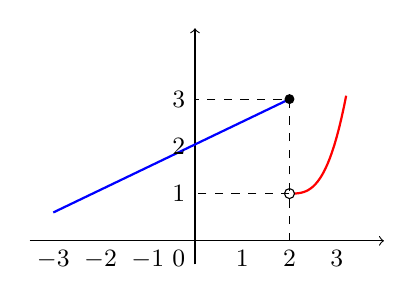
\begin{tikzpicture}[scale=0.6]
    \draw[->] (-3.5,0) -- (4,0); \draw[->] (0,-0.5) -- (0,4.5);
    \draw[thick,blue] (-3,0.6) -- (2,3);
    \draw[thick,red,domain=2:3.2] plot (\x,{1+1.2*(\x-2)^3});
    \fill (2,3) circle (3pt); \draw[fill=white] (2,1) circle (3pt);
    \draw[dashed] (2,0) -- (2,3) -- (0,3); \draw[dashed] (2,1) -- (0,1);
    \foreach \x in {-3,-2,-1,1,2,3} \node[below] at (\x,0) {\small $\x$};
    \foreach \y in {1,2,3} \node[left] at (0,\y) {\small $\y$};
    \node[below left] at (0,0) {\small $0$};
  \end{tikzpicture}
  \end{center}
  \ans
  $\displaystyle\lim_{x \to 2^+} f(x) = 1$ និង $\displaystyle\lim_{x \to 2^-} f(x) = 3$ ។
\end{enumerate}
